\documentclass[slovene,11pt,a4paper]{article}
\usepackage[margin=2cm,bottom=3cm,foot=1.5cm]{geometry}

\setlength{\parindent}{0pt}
\setlength{\parskip}{0.5ex}

\usepackage[pdftex]{graphicx}
\DeclareGraphicsExtensions{.pdf,.png}


\usepackage{amsmath}
\usepackage{amsfonts}
\usepackage{mathrsfs}
\usepackage[usenames]{color}
\usepackage[slovene]{babel}
\usepackage[utf8]{inputenc}
\usepackage{siunitx}
\usepackage{subcaption}
\usepackage{float}

\def\phi{\varphi}
\def\eps{\varepsilon}
\def\theta{\vartheta}

\newcommand{\thisyear}{2025/26}

\renewcommand{\Re}{\mathop{\rm Re}\nolimits}
\renewcommand{\Im}{\mathop{\rm Im}\nolimits}
\newcommand{\Tr}{\mathop{\rm Tr}\nolimits}
\newcommand{\diag}{\mathop{\rm diag}\nolimits}
\newcommand{\dd}{\,\mathrm{d}}
\newcommand{\ddd}{\mathrm{d}}
\newcommand{\ii}{\mathrm{i}}
\newcommand{\lag}{\mathcal{L}\!}
\newcommand{\ham}{\mathcal{H}\!}
\newcommand{\four}[1]{\mathcal{F}\!\left(#1\right)}
\newcommand{\bigO}[1]{\mathcal{O}\!\left(#1\right)}
\newcommand{\sh}{\mathop{\rm sinh}\nolimits}
\newcommand{\ch}{\mathop{\rm cosh}\nolimits}
\renewcommand{\th}{\mathop{\rm tanh}\nolimits}
\newcommand{\erf}{\mathop{\rm erf}\nolimits}
\newcommand{\erfc}{\mathop{\rm erfc}\nolimits}
\newcommand{\sinc}{\mathop{\rm sinc}\nolimits}
\newcommand{\rect}{\mathop{\rm rect}\nolimits}
\newcommand{\ee}[1]{\cdot 10^{#1}}
\newcommand{\inv}[1]{\left(#1\right)^{-1}}
\newcommand{\invf}[1]{\frac{1}{#1}}
\newcommand{\sqr}[1]{\left(#1\right)^2}
\newcommand{\half}{\frac{1}{2}}
\newcommand{\thalf}{\tfrac{1}{2}}
\newcommand{\pd}{\partial}
\newcommand{\Dd}[3][{}]{\frac{\ddd^{#1} #2}{\ddd #3^{#1}}}
\newcommand{\Pd}[3][{}]{\frac{\pd^{#1} #2}{\pd #3^{#1}}}
\newcommand{\avg}[1]{\left\langle#1\right\rangle}
\newcommand{\norm}[1]{\left\Vert #1 \right\Vert}
\newcommand{\braket}[2]{\left\langle #1 \vert#2 \right\rangle}
\newcommand{\obraket}[3]{\left\langle #1 \vert #2 \vert #3 \right \rangle}
\newcommand{\hex}[1]{\texttt{0x#1}}

\renewcommand{\iint}{\mathop{\int\mkern-13mu\int}}
\renewcommand{\iiint}{\mathop{\int\mkern-13mu\int\mkern-13mu\int}}
\newcommand{\oiint}{\mathop{{\int\mkern-15mu\int}\mkern-21mu\raisebox{0.3ex}{$\bigcirc$}}}

\newcommand{\wunderbrace}[2]{\vphantom{#1}\smash{\underbrace{#1}_{#2}}}

\renewcommand{\vec}[1]{\overset{\smash{\hbox{\raise -0.42ex\hbox{$\scriptscriptstyle\rightharpoonup$}}}}{#1}}
\newcommand{\bec}[1]{\mathbf{#1}}



\title{
\sc\large Matematično-fizikalni praktikum \thisyear\\
\bigskip
\bf\Large 1.~naloga: Airyjevi funkciji
}
\author{Samo Krejan, 28231092}
\date{}

\newcommand{\Ai}{\mathrm{Ai}}
\newcommand{\Bi}{\mathrm{Bi}}
\newcommand{\bi}[1]{\hbox{\boldmath{$#1$}}}
\newcommand{\bm}[1]{\hbox{\underline{$#1$}}}


\begin{document}
\maketitle
\vspace{-1cm}

\section{Uvod}
\label{uvod}

Airyjevi funkciji $\Ai$ in $\Bi$ % #TODO: add figure
se v fiziki pojavljata predvsem v optiki in kvantni mehaniki
\cite{Airy_use}.  Definirani sta kot neodvisni rešitvi enačbe
%
\begin{equation*}
  y''(x) -xy(x) = 0
\end{equation*}
%
in sta predstavljivi v integralski obliki
%
\begin{equation*}
  \Ai(x) = \frac{1}{\pi} \int_0^\infty \cos (t^3/3 + x t) \dd t \>,\quad
  \Bi(x) = \frac{1}{\pi} \int_0^\infty \left[ \mathrm{e}^{-t^3/3 + x t}
  + \sin (t^3/3 + x t) \right] \dd t \>.
\end{equation*}
%


Za majhne $x$ lahko funkciji $\Ai$ in $\Bi$ izrazimo
z Maclaurinovima vrstama
%
\begin{equation*}
  \Ai(x) = \alpha f(x) - \beta g(x)\>,\qquad
  \Bi(x) = \sqrt{3}\, \Bigl[\alpha f (x) + \beta g(x) \Bigr]\>,
\end{equation*}
kjer v $x=0$ veljata zvezi
%
$\alpha = \Ai(0) = \Bi(0)/\sqrt{3}\approx 0.355028053887817239$ in
$\beta = -\Ai'(0) = \Bi'(0)/\sqrt{3}\approx 0.258819403792806798$.
Vrsti za $f$ in $g$ sta
\begin{equation*}
  f(x) = \sum_{k=0}^\infty
  \left(\frac{1}{3}\right)_k \frac{3^k x^{3k}}{(3k)!} \>, \qquad
  g(x) = \sum_{k=0}^\infty
  \left(\frac{2}{3}\right)_k \frac{3^k x^{3k+1}}{(3k+1)!} \>,
\end{equation*}
kjer je
\begin{equation*}
  (z)_n = \Gamma(z+n)/\Gamma(z) \>, \qquad (z)_0 = 1 \>.
\end{equation*}

Za velike vrednosti $|x|$ Airyjevi funkciji aproksimiramo
z njunima asimp\-tot\-ski\-ma razvojema.  Z novo spremenljivko
$\xi=\frac{2}{3} |x|^{3/2}$ in asimptotskimi vrstami
%
\begin{equation*}
  L(z) \sim \sum_{s=0}^\infty \frac{u_s}{z^s}\>,\qquad
  P(z) \sim \sum_{s=0}^\infty (-1)^s \frac{u_{2s}}{z^{2 s}}\>,\qquad
  Q(z) \sim \sum_{s=0}^\infty (-1)^s \frac{u_{2s+1}}{z^{2 s+1}}\>,
\end{equation*}
s koeficienti
\begin{equation*}
u_s = \frac{ \Gamma(3s + \frac{1}{2})}
        {54^s s!\, \Gamma(s + \frac{1}{2}) }
\end{equation*}
za velike pozitivne $x$ izrazimo
%
\begin{equation*}
\Ai(x)\sim  \frac{\mathrm{e}^{-\xi}}{2\sqrt{\pi} x^{1/4}} \, L(-\xi) \>, \qquad
\Bi(x)\sim  \frac{\mathrm{e}^{\xi}} { \sqrt{\pi} x^{1/4}} \, L(\xi)\>,
\end{equation*}
%
za po absolutni vrednosti velike negativne $x$ pa
%
%
\begin{align*}
    \Ai(x)&\sim  \frac{1}{\sqrt{\pi} (-x)^{1/4}}
    \Bigl[ \phantom{-}\sin(\xi-\pi/4) \, Q(\xi)
                    + \cos(\xi-\pi/4) \, P(\xi)\Bigr] \>, \\
    \Bi(x)&\sim  \frac{1}{\sqrt{\pi} (-x)^{1/4}}
    \Bigl[ - \sin(\xi-\pi/4) \, P(\xi)
      + \cos(\xi-\pi/4) \, Q(\xi)\Bigr]\>.
\end{align*}


\section{Naloga}

Z uporabo kombinacije Maclaurinove vrste in asimptotskega
razvoja poišči čim učinkovitejši postopek za izračun
vrednosti Airyjevih funkcij $\Ai$ in $\Bi$ na vsej real\-ni osi
z {\bf absolutno} napako, manjšo od $10^{-10}$. Enako naredi tudi z {\bf relativno} napako in ugotovi,
ali je tudi pri le-tej dosegljiva natančnost, manjša od $10^{-10}$.
Pri oceni napak si po\-ma\-gaj s programi, ki znajo računati s poljubno
natančnostjo, na primer z {\sc Mathematico} in/ali paketi {\sc mpmath} in {\sc decimal} v programskem
jeziku {\sc Python}.

\subsection{Maclaurinov približek}


Člene vrst $f$ in $g$ zapišemo rekurzivno, in $n$-ti člen zapišemo kot produkt prejšnjega in količnika:

\begin{equation*}
  f_n = f_{n-1} \cdot \frac{f_n}{f_{n-1}} = f_{n-1} \cdot \frac{x^3}{3n(3n - 1)} \>, \qquad f_0 = 1
\end{equation*}

\begin{equation*}
  g_n = g_{n-1} \cdot \frac{g_n}{g_{n-1}} = g_{n-1} \cdot \frac{x^3}{3n(3n + 1)} \>, \qquad g_0 = x
\end{equation*}
Dobljene rezultate bomo skozi nalogo primerjali z vgrajenima funkcijama $mpmath.airyai()$ in $mpmath.airybi()$, ki gotovo od dejanske vrednosti odstopata manj kot $\ee{-20}$ \cite{airy_luka}.

\begin{figure}[ht]
\begin{center}
  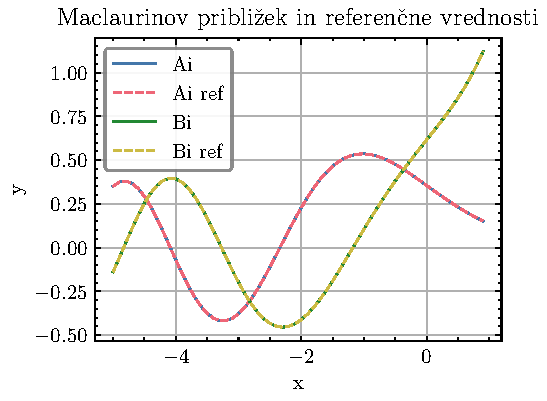
\includegraphics[width=10cm]{graphs/mac_draw.pdf}
  \caption{Maclaurinov približek $Ai$ in $Bi$ primerjan z vgrajenima funkcija}
  \label{fig: mac_draw}
\end{center}
\end{figure}

\begin{figure}[ht]
  \centering
  \begin{minipage}{0.42\textwidth}
    \centering
    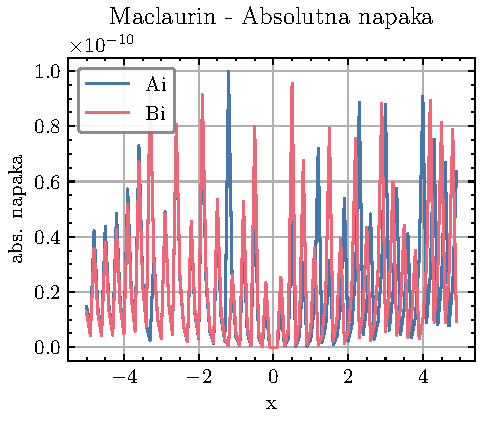
\includegraphics[width=\linewidth]{graphs/mac_abs_err.pdf}
    % \caption{First plot.}
    % \label{fig:plot1}
  \end{minipage}\hfill
  \begin{minipage}{0.48\textwidth}
    \centering
    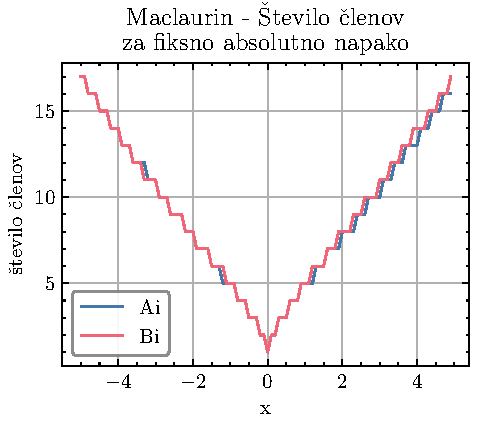
\includegraphics[width=\linewidth]{graphs/mac_abs_err_n.pdf}
    % \caption{Second plot.}
    % \label{fig:plot2}
  \end{minipage}
  \caption{Absolutna napaka naše implementacije in število členov potrebnih, da le ta ostane pod $10^{-10}$. Iz grafov vidimo, da se napaka sicer z oddaljenostjo od izhodišča strmo veča, a vsakič ko bi le ta zgrešila željeno natančnost se vrsti doda en člen. To pojasni močno zobničasto naravo napake.}
  \label{fig: mac_abs_err}
\end{figure}


\begin{figure}[ht]
  \centering
  \begin{minipage}{0.42\textwidth}
    \centering
    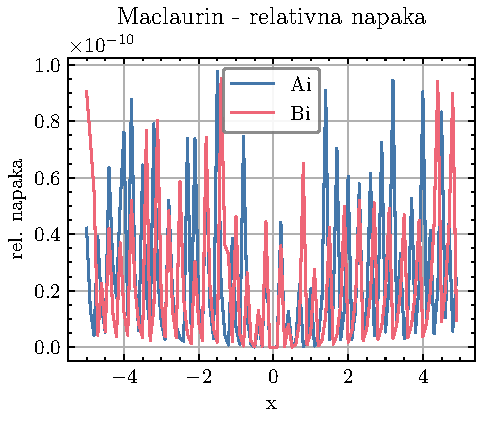
\includegraphics[width=\linewidth]{graphs/mac_rel_err.pdf}
    % \caption{First plot.}
    % \label{fig:plot1}
  \end{minipage}\hfill
  \begin{minipage}{0.48\textwidth}
    \centering
    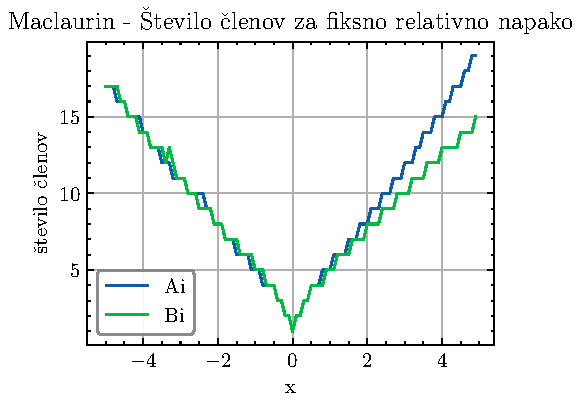
\includegraphics[width=\linewidth]{graphs/mac_rel_err_n.pdf}
    % \caption{Second plot.}
    % \label{fig:plot2}
  \end{minipage}
  \caption{Relativna napaka in potrebno število členov vrste za doseg te napake. Karakteristika je ekvivalentna tisti pri absolutni napaki. Tudi potrebno število členov se ne spremeni znatno, le pri večjih pozitivnih vrednostih opazimo, da potrebujemo vedno več členov za funkcijo $Ai$.}
  \label{fig: mac_rel_err}
\end{figure}

Že na prvi pogled, ko grafiramo dobljene vrednosti za obe funkciji in jih primerjamo z vgrajenima funkcijama vidimo (slika: \ref{fig: mac_draw}), da je Maclaurinov približek precej uspešen. To še dodatno potrdita sliki \ref{fig: mac_abs_err} in \ref{fig: mac_rel_err}, kjer vidimo, da nam je na območju $(-4, 4)$ uspelo \textit{ujeti} tako željeno absolutno kot relativno napako z manj kot dvajsetimi členi.

Zanimivost, ki se mi jo zdi vredno omeniti lahko opazimo na desni sliki \ref{fig: mac_rel_err}, kjer vidimo, da se število potrebnih členov funkcije $Ai$ hitro veča. To je seveda smiselno, ko pomislimo, da tam $Ai$ dosega vrednosti zelo blizu $0$ in je tako seveda za enako relativno natančnost, potrebna veliko boljša absolutna natančnost.
\newpage



\subsection{Asimptotski približek za velike negativne $x$}

Člene vrst razvoja funcij $P$ in $Q$ prav tako, kot pri Maclaurinovem razvoju zapišemo rekurzivno, saj tako močno izboljšamo hitrost algoritma.

\begin{equation*}
  p_n = p_{n-1} \cdot \frac{p_n}{p_{n-1}} = - p_{n-1} \cdot \frac{(6n - 1/2)(6n - 5/2)(6n - 7/2)(6n - 11/2)}{(2n - 1)(2n)18^2x^2} \>, \qquad p_0 = 1
\end{equation*}

\begin{equation*}
  q_n = q_{n-1} \cdot \frac{q_n}{q_{n-1}} = - q_{n-1} \cdot \frac{(6n - 1/2)(6n - 5/2)(6n + 1/2)(6n + 5/2)}{(2n + 1)(2n)18^2x^2} \>, \qquad q_0 = \frac{5}{72x}
\end{equation*}

Pri obeh asimptotskih priblizkih moramo sicer paziti, da ne uporabimo preveč členov v vrsti. Izkaže se namreč, da se začne napaka pri nekem členu nazaj večati. Iz tega razloga vrsto odrežemo, ko naslednji člen postane večji od prejšnjega. Poraja se vprašanje, če je to res najboljša meja za \textit{odsek} vrste: 
\begin{quote}
  Odgovor je da je to tok blizu, da je praktično optimalno. (Jakob Kralj, 2025)
\end{quote}
\newpage

\begin{figure}[h]
  \centering
  \begin{minipage}{0.48\textwidth}
    \centering
    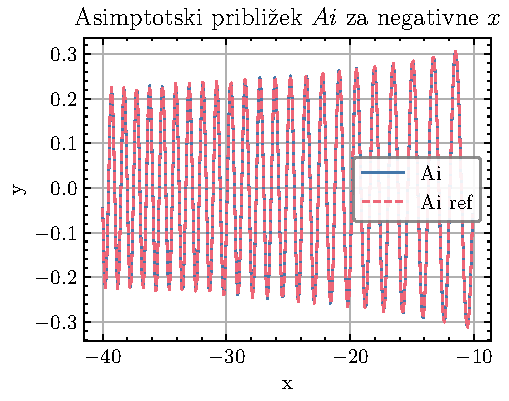
\includegraphics[width=\linewidth]{graphs/neg_draw_ai.pdf}
    % \caption{First plot.}
    % \label{fig:plot1}
  \end{minipage}\hfill
  \begin{minipage}{0.48\textwidth}
    \centering
    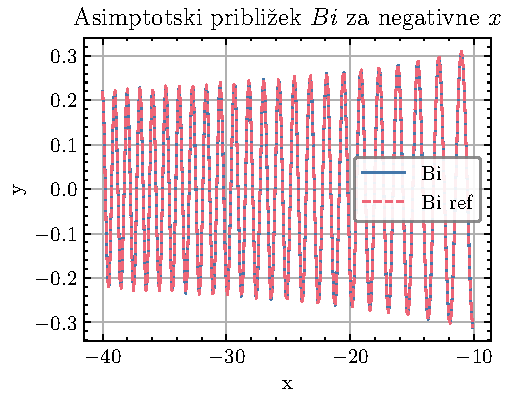
\includegraphics[width=\linewidth]{graphs/neg_draw_bi.pdf}
    % \caption{Second plot.}
    % \label{fig:plot2}
  \end{minipage}
  \caption{Asimptotski približek za $Ai$ (levo) in $Bi$ (desno) primerjan z vgrajenima funkcijama.}
  \label{fig: neg_draw}
\end{figure}


\begin{figure}[h]%#TODO fig size
  \centering
  \begin{minipage}{0.48\textwidth}
    \centering
    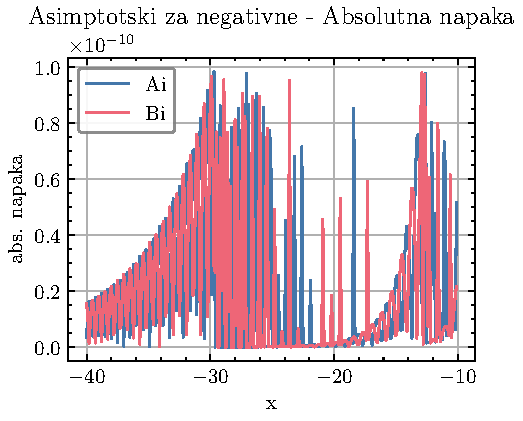
\includegraphics[width=\linewidth]{graphs/neg_abs_err.pdf}
    % \caption{First plot.}
    % \label{fig:plot1}
  \end{minipage}\hfill
  \begin{minipage}{0.48\textwidth}
    \centering
    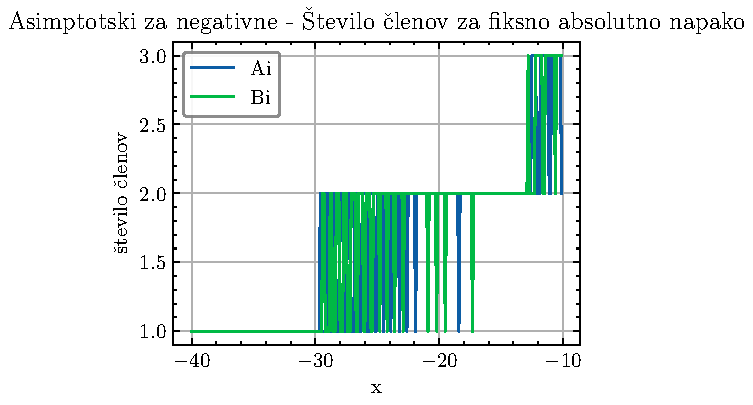
\includegraphics[width=\linewidth]{graphs/neg_abs_err_n.pdf}
    % \caption{Second plot.}
    % \label{fig:plot2}
  \end{minipage}
  \caption{Absolutna napaka (levo) in število členov asimptotske vrste potrebnih za doseg le te. Zanimivo vidimo, da bolj kot je negativen $x$ manj manjša je napaka in je zato posledično potrebnih manj členov.}
  \label{fig: neg_abs}
\end{figure}


\begin{figure}[H]%#TODO fig size
  \centering
  \begin{minipage}{0.42\textwidth}
    \centering
    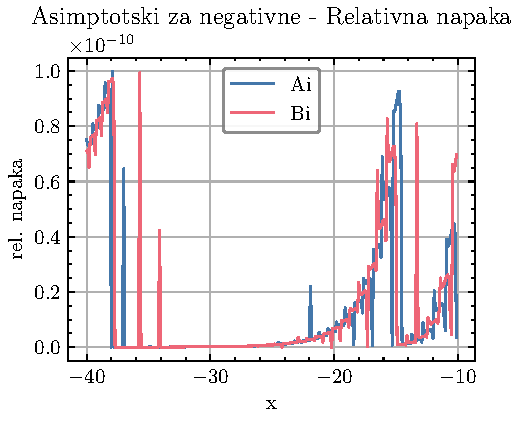
\includegraphics[width=\linewidth]{graphs/neg_rel_err.pdf}
    % \caption{First plot.}
    % \label{fig:plot1}
  \end{minipage}\hfill
  \begin{minipage}{0.55\textwidth}
    \centering
    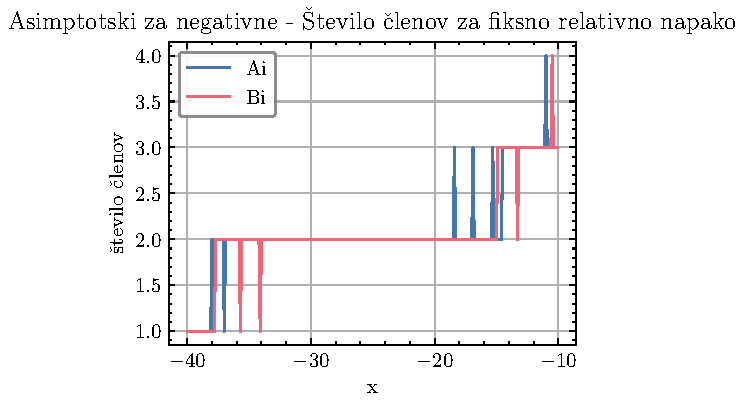
\includegraphics[width=\linewidth]{graphs/neg_rel_err_n.pdf}
    % \caption{Second plot.}
    % \label{fig:plot2}
  \end{minipage}
  \caption{Relativna napaka (levo) in število členov potrebnih za doseg le te (desno). Sama karakteristika je seveda zelo podobna kot pri absolutni napaki (glej sliko \ref{fig: neg_abs}) a lahko opazimo, da je v splošnem za konstantno relativno napako potrebnih nekoliko več členov}
  \label{fig: neg_rel}
\end{figure}




\newpage
\subsection{Asimptotski približek za velike pozitivne $x$}


Za velike pozitivne $x$ uporabimo vrsto $L$ opisano v poglavju \ref{uvod}. Katere člene lahko spet zapišemo rekurzivno za potrebe optimizacije:

\begin{equation*}
  l_n = l_{n-1} \cdot \frac{l_n}{l_{n-1}} = l_{n-1} \cdot \frac{(3n + 1/2)(3n + 5/2)}{(n + 1)18x} \>, \qquad l_0 = 1
\end{equation*}

Pristop od tu naprej je seveda ekvivalenten tistemu za velike negativne $x$.

\begin{figure}[h]
  \centering
  \begin{minipage}{0.48\textwidth}
    \centering
    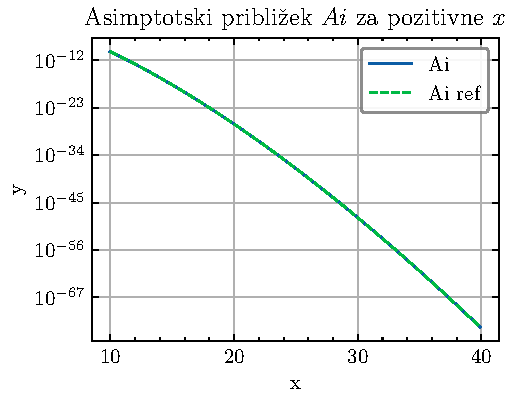
\includegraphics[width=\linewidth]{graphs/pos_draw_ai.pdf}
    % \caption{First plot.}
    % \label{fig:plot1}
  \end{minipage}\hfill
  \begin{minipage}{0.48\textwidth}
    \centering
    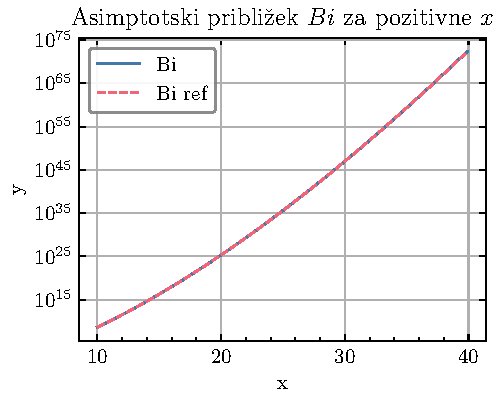
\includegraphics[width=\linewidth]{graphs/pos_draw_bi.pdf}
    % \caption{Second plot.}
    % \label{fig:plot2}
  \end{minipage}
  \caption{Asimptotski približek za $Ai$ (levo) in $Bi$ (desno) primerjan z vgrajenima funkcijama.}
  \label{fig: pos_draw}
\end{figure}


\begin{figure}[H]
  \centering

  % Row 1
  \begin{subfigure}{0.48\textwidth}
    \centering
    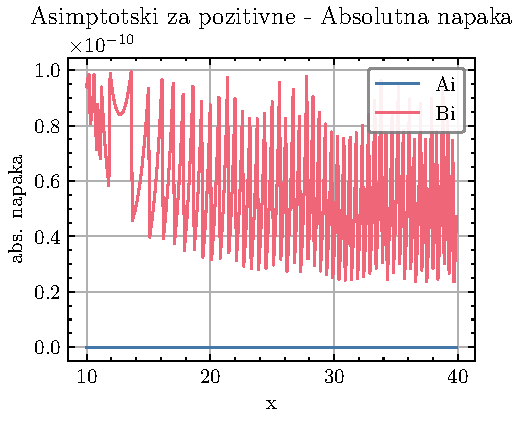
\includegraphics[width=\linewidth]{graphs/pos_abs_err.pdf}
    \caption{First subfigure.}
    \label{fig:a}
  \end{subfigure}\hfill
  \begin{subfigure}{0.48\textwidth}
    \centering
    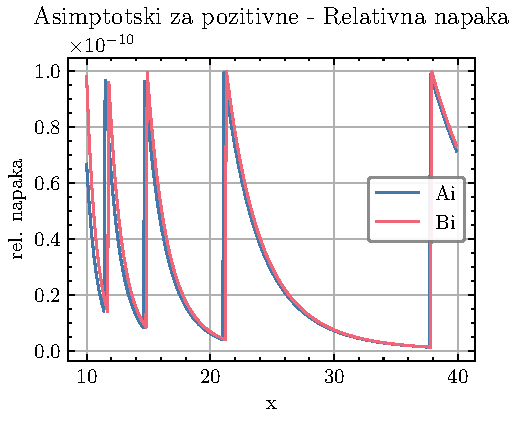
\includegraphics[width=\linewidth]{graphs/pos_rel_err.pdf}
    \caption{Second subfigure.}
    \label{fig:b}
  \end{subfigure}

  % Row 2
  \begin{subfigure}{0.48\textwidth}
    \centering
    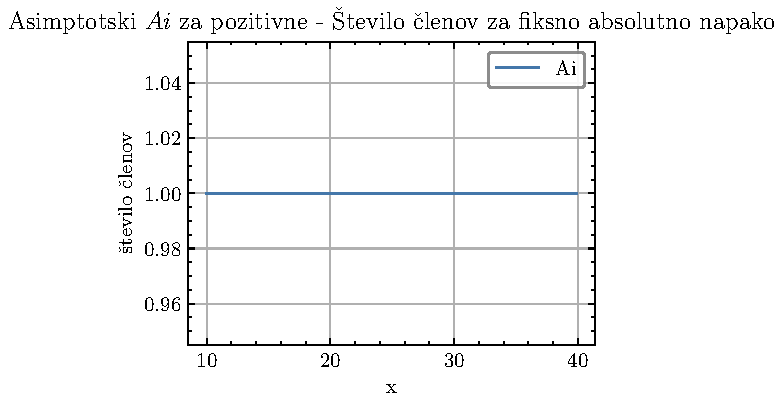
\includegraphics[width=\linewidth]{graphs/pos_abs_err_n_ai.pdf}
    \caption{Third subfigure.}
    \label{fig:c}
  \end{subfigure}\hfill
  \begin{subfigure}{0.48\textwidth}
    \centering
    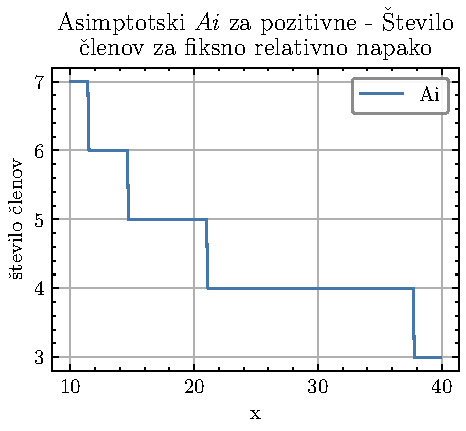
\includegraphics[width=\linewidth]{graphs/pos_rel_err_n_ai.pdf}
    \caption{Fourth subfigure.}
    \label{fig:d}
  \end{subfigure}

  % Row 3
  \begin{subfigure}{0.48\textwidth}
    \centering
    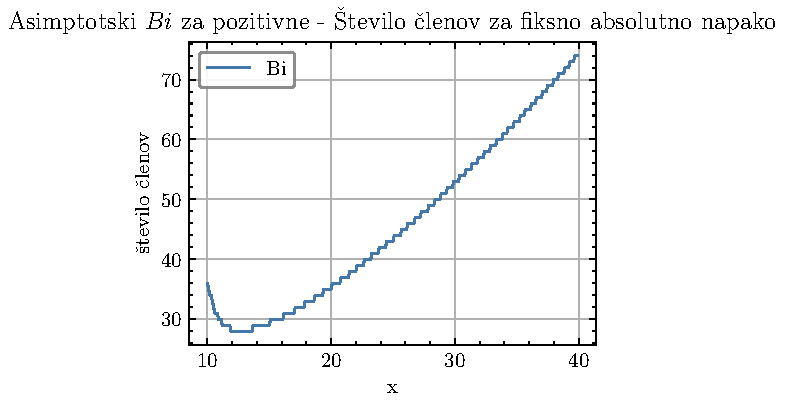
\includegraphics[width=\linewidth]{graphs/pos_abs_err_n_bi.pdf}
    \caption{Third subfigure.}
    % \label{fig:c}
  \end{subfigure}\hfill
  \begin{subfigure}{0.48\textwidth}
    \centering
    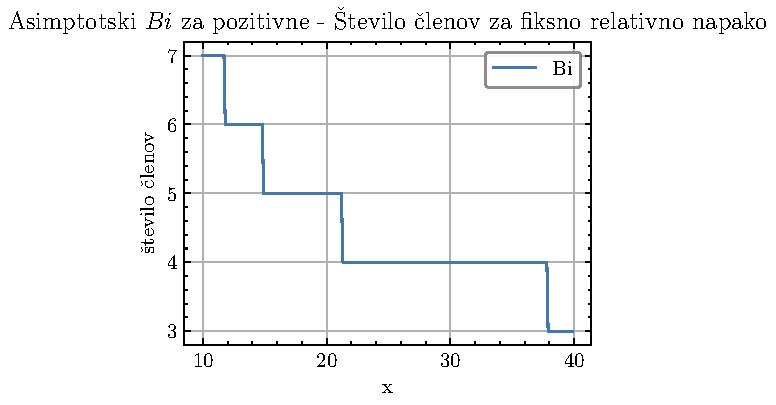
\includegraphics[width=\linewidth]{graphs/pos_rel_err_n_Bi.pdf}
    \caption{Fourth subfigure.}
    % \label{fig:d}
  \end{subfigure}

  \caption{Overview of all four cases: (a)–(d).}
  \label{fig:fourplots}
\end{figure}


\section{Dodatna naloga}

Ničle funkcije $\Ai$ pogosto srečamo v matematični
analizi pri določitvi intervalov ničel specialnih funkcij
in ortogonalnih polinomov \cite{1_szego} ter v fiziki pri računu
energijskih spektrov kvantnomehanskih sistemov \cite{1_landauQM}.
Poišči prvih sto ničel $\{a_s\}_{s=1}^{100}$ Airyjeve
funkcije $\Ai$ in prvih sto ničel $\{b_s\}_{s=1}^{100}$
funkcije $\Bi$ pri $x<0$ ter dobljene vrednosti primerjaj s formulama
%
\begin{equation*}
  a_s = - f \left( \frac{3\pi(4s-1)}{8} \right) \>, \qquad
  b_s = - f \left( \frac{3\pi(4s-3)}{8} \right) \>, \qquad s = 1,2,\ldots \>,
\end{equation*}
%
kjer ima funkcija $f$ asimptotski razvoj \cite{1_abram}
%
\begin{equation*}
  f(z) \sim z^{2/3} \left(
  1 + \frac{5}{48} \, z^{-2}
  -\frac{5}{36} \, z^{-4}
  +\frac{77125}{82944} \, z^{-6}
  -\frac{108056875}{6967296} \, z^{-8} + \ldots\right) \>.
\end{equation*}


\bibliographystyle{plain}
\bibliography{references}


\end{document}